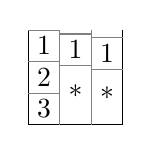
\begin{tikzpicture}
  %%%%%%%%%%%%%The first bin%%%%%%%%%%%%%%%%%%%%%%
  \draw (0,1.2) -- (0,0) -- (1.2,0)--(1.2,1.2);
  \draw[gray] (0.4,0) -- (0.4,1.2);
  \draw[gray] (0.8,0) -- (0.8,1.2);
  \draw[gray] (0,1.2) -- (0.4,1.2);
  \draw[gray] (0,0.8) -- (0.4,0.8);
  \draw[gray] (0,0.4) -- (0.4,0.4);
  \draw[gray] (0.4,1.15) -- (0.8,1.15);
  \draw[gray] (0.4,0.75) -- (0.8,0.75);
  \draw[gray] (0.8,1.1) -- (1.2,1.1);
  \draw[gray] (0.8,0.7) -- (1.2,0.7);

  \draw (0.2,1) node {1};
  \draw (0.2,0.6) node {2};
  \draw (0.2,0.2) node {3};
  \draw (0.6,0.95) node {1};
  \draw (1,0.9) node {1};
  \draw (0.6,0.375) node {*};
  \draw (1,0.35) node {*};
\end{tikzpicture}
\quad
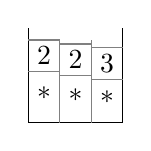
\begin{tikzpicture}
  %%%%%%%%%%%%%The second bin%%%%%%%%%%%%%%%%%%%%%%
  \draw (0,1.2) -- (0,0) -- (1.2,0)--(1.2,1.2);
  \draw[gray] (0.4,0) -- (0.4,1.05);
  \draw[gray] (0.8,0) -- (0.8,1.05);
  \draw[gray] (0,1.05) -- (0.4,1.05);
  \draw[gray] (0,0.65) -- (0.4,0.65);
  \draw[gray] (0.4,1) -- (0.8,1);
  \draw[gray] (0.4,0.6) -- (0.8,0.6);
  \draw[gray] (0.8,0.95) -- (1.2,0.95);
  \draw[gray] (0.8,0.55) -- (1.2,0.55);

  \draw (0.2,0.85) node {2};
  \draw (0.2,0.325) node {*};
  \draw (0.6,0.8) node {2};
  \draw (0.6,0.3) node {*};
  \draw (1,0.75) node {3};
  \draw (1,0.275) node {*};
\end{tikzpicture}
\quad
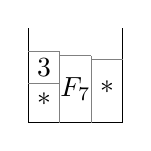
\begin{tikzpicture}
  %%%%%%%%%%%%%The third bin%%%%%%%%%%%%%%%%%%%%%%
  \draw (0,1.2) -- (0,0) -- (1.2,0)--(1.2,1.2);
  \draw[gray] (0.4,0) -- (0.4,0.9);
  \draw[gray] (0.8,0) -- (0.8,0.85);
  \draw[gray] (0,0.9) -- (0.4,0.9);
  \draw[gray] (0,0.5) -- (0.4,0.5);
  \draw[gray] (0.4,0.85) -- (0.8,0.85);
  \draw[gray] (0.8,0.8) -- (1.2,0.8);

  \draw (0.2,0.7) node {3};
  \draw (0.2,0.25) node {*};
  \draw (0.6,0.425) node {$F_7$};
  \draw (1,0.4) node {*};
\end{tikzpicture}
